% Created 2015-03-18 ons 12:03
\documentclass[colorlinks=true,linkcolor=blue]{article}
\usepackage[utf8]{inputenc}
\usepackage[T1]{fontenc}
\usepackage{fixltx2e}
\usepackage{graphicx}
\usepackage{longtable}
\usepackage{float}
\usepackage{wrapfig}
\usepackage{rotating}
\usepackage[normalem]{ulem}
\usepackage{amsmath}
\usepackage{textcomp}
\usepackage{marvosym}
\usepackage{wasysym}
\usepackage{amssymb}
\usepackage{hyperref}
\tolerance=1000
\usepackage[top=1in,bottom=1in,left=1.2in,right=1.2in]{geometry}
\usepackage{pgf}
\usepackage{tikz}
\usetikzlibrary{arrows,automata}
\author{Sander Jespersen, Mathias Melgaard Andersen, Anders Roland Nielsen, \\ Andreas Berre Eriksen, Kent Munthe Caspersen \& Mikkel Alexander Madsen}
\date{\today}
\title{aMI Handin assignments}
\hypersetup{
  pdfkeywords={},
  pdfsubject={},
  pdfcreator={Emacs 24.4.1 (Org mode 8.2.10)}}
\begin{document}

\maketitle

\section{Water tank}
\label{sec-1}
\subsection{Baysian network}
\label{sec-1-1}
Indsæt figur fra Genie image.

\subsection{Suitable conditional probability distribution}
\label{sec-1-2}
Hvis ventil er åben fanger den stortset altid der er flow, hvis den er lukket laver den oftere fejl.


\subsection{Simulation}
\label{sec-1-3}
We assume that only the controller has access to the water level sensor, and thus we can not manually read the water level through the sensor.

\section{Matlab}
\label{sec-2}
\subsection{Forward-backward algorithm}
\label{sec-2-1}
The changes we did to the given code was as follows:
\begin{itemize}
\item In the HMM class we added a backwardMessages
\item We initialised it to NaN when a HMM object was created
\end{itemize}
\begin{verbatim}
backwardMessages;

function obj = HMM(priorModel, transModel, sensorModel)
  ...
  obj.backwardMessages = NaN;
end
\end{verbatim}

The code below is our implementation of the backward part of the algorithm. The linebreak in the code is not present in the actual code but was done to fit on the page.

\begin{verbatim}
function obj = backward(obj, data)
  totalTime = length(data);

  obj.backwardMessages=zeros(obj.noHidden,totalTime+1);           

  obj.backwardMessages(:,totalTime+1) = 1;
    for t=totalTime:-1:1,
      obj.backwardMessages(:,t) 
      = obj.transModel*obj.sensorModel{data(t)}*obj.backwardMessages(:,t+1);
      obj.backwardMessages(:,t) 
      = obj.backwardMessages(:,t)./sum(obj.backwardMessages(:,t));
    end
end
\end{verbatim}

The result of running the our function on the given demo that forward was run on gives the following result:

\begin{center}
\begin{tabular}{rrrrrr}
0.6469 & 0.5923 & 0.3763 & 0.6533 & 0.6273 & 1.0000\\
0.3531 & 0.4077 & 0.6237 & 0.3467 & 0.3727 & 1.0000\\
\end{tabular}
\end{center}

\subsection{HMM for exercise 1}
\label{sec-2-2}
\begin{verbatim}
Trans = [ 0.8, 0.2; 
	  0.2, 0.8 ];
Prio = [ 0.6, 0.4 ]';
Sens = [ 0.02, 0.21; 
	 0.18, 0.49; 
	 0.08, 0.09; 
	 0.72, 0.21 ]';

% 1=yes+red, 2=yes+not red,  3=no+red, 4=no+not red
Dat = [ 4, 2, 1 ];

newhmm = HMM(Prio, Trans, Sens);
newhmm = newhmm.forward(Dat);
newhmm = newhmm.backward(Dat);

disp('Forward:');
disp(newhmm.forwardMessages);
disp('Backward:');
disp(newhmm.backwardMessages);
\end{verbatim}

\subsection{Implementation of HMM}
\label{sec-2-3}
\begin{itemize}
\item Forward:
\begin{center}
\begin{tabular}{rrr}
0.8372 & 0.4643 & 0.0804\\
0.1628 & 0.5357 & 0.9196\\
\end{tabular}
\end{center}

\item Backward:
\end{itemize}
\begin{center}
\begin{tabular}{rrrr}
0.5325 & 0.2661 & 0.2522 & 1.0000\\
0.4675 & 0.7339 & 0.7478 & 1.0000\\
\end{tabular}
\end{center}
\section{Exercise 3}
\label{sec-3}
\subsection{Umbrella}
\label{sec-3-1}
\begin{itemize}
\item By calculating the likelihood of the models correctness and the one with the highest likelihood is the most reliable model:
\begin{itemize}
\item 0.7 $\cdot$ 0.7 $\cdot$ 0.7 $\cdot$ 0.3 $\cdot$ 0.7 $\cdot$ 0.7 $\cdot$ 0.3 $\cdot$ 0.3 $\cdot$ 0.7 = 0.003176523
\item 0.6 $\cdot$ 0.6 $\cdot$ 0.6 $\cdot$ 0.4 $\cdot$ 0.8 $\cdot$ 0.8 $\cdot$ 0.2 $\cdot$ 0.4 $\cdot$ 0.8 = 0.003538944
\end{itemize}
\item Matlab
\end{itemize}
\begin{verbatim}
function p = SSP(obj, sequence)
  p = 1;
  for t=2:length(sequence),
    transition = obj.transModel(sequence(t-1),sequence(t));
    p = p * transition;                
  end
end
\end{verbatim}
\begin{itemize}
\item MATLAB gave us the same results as the manual calculations of the likelihood.
\end{itemize}


\subsection{Water tank}
\label{sec-3-2}
\begin{itemize}
\item Kalman Filter
\end{itemize}
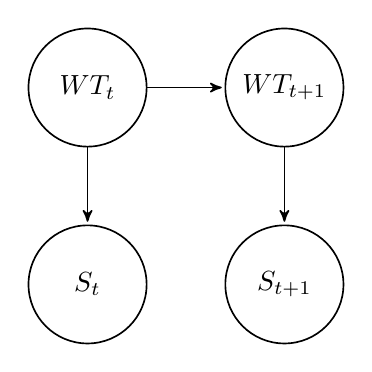
\begin{tikzpicture}[->,>=stealth',shorten >=1pt,auto,node distance=2.5cm, semithick]

\node[state, minimum size=1.5cm] (B) {$WT_t$};
\node[state, minimum size=1.5cm] (C) [below of = B] {$S_t$};
\node[state, minimum size=1.5cm] (D) [right of = B] {$WT_{t+1}$};
\node[state, minimum size=1.5cm] (E) [right of = C] {$S_{t+1}$};

\path (B) edge (D)
      (B) edge (C)
      (D) edge (E);

\end{tikzpicture}
\begin{enumerate}
\item $WT_{t+1} = \mathcal{N}(WT_t,1)$
\item $S_t = \mathcal{N}(WT_t,1.5)$
\end{enumerate}

\begin{itemize}
\item Filtered estimates:
\end{itemize}
% Emacs 24.4.1 (Org mode 8.2.10)
\end{document}